\section{Design Space Map By Session}
 The ``unfolded'' version of Figure 7 is presented here. Each graph corresponds to data from a session. 
 
\begin{figure*}[!ht] 
    \centering
    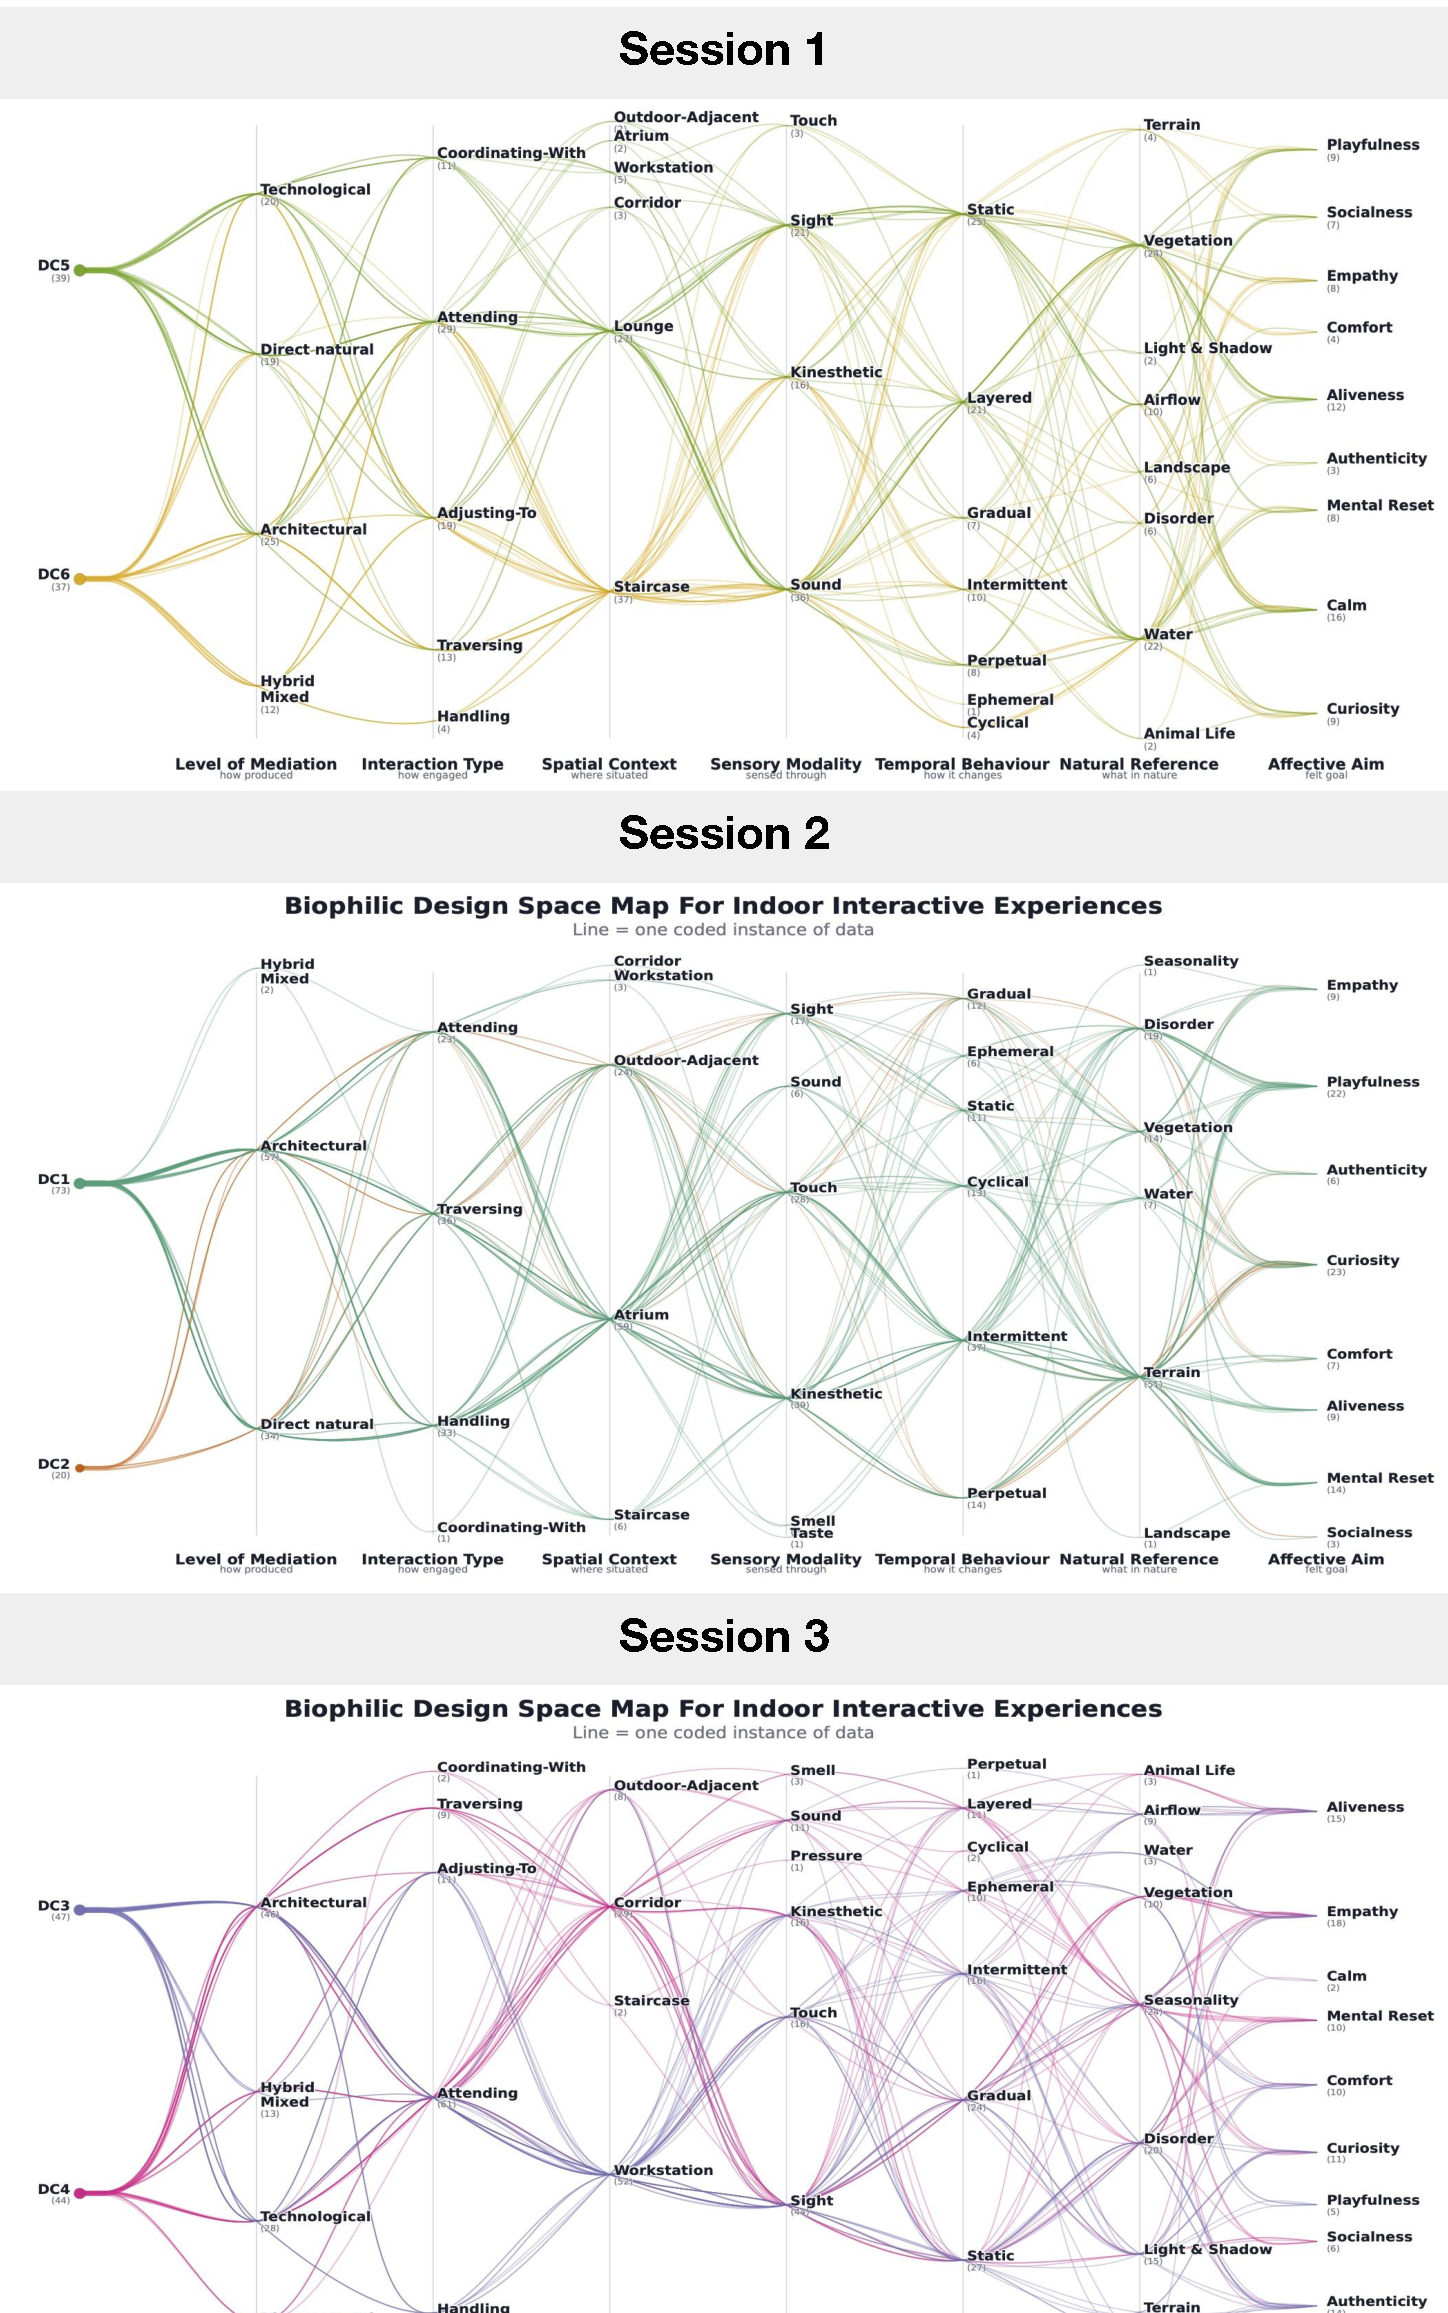
\includegraphics[width=0.68\linewidth]{images/design-space-bysessions.pdf}
    \caption{Overview of the design space by session. Design concepts DC1–DC2 originate from Session 1, which explored the breadth of biophilic interactive experiences; DC3–DC4 are from Session 2, which focused on translating experiential qualities into interaction mechanisms; and DC5–DC6 are from Session 3, which foregrounded sound as a biophilic modality.}
    \Description{An overview diagram of the biophilic design space organised by session, showing that design concepts DC1–DC2 originate from Session 1 exploring the breadth of biophilic experiences, DC3–DC4 from Session 2 focusing on translating experiences into interaction mechanisms, and DC5–DC6 from Session 3 foregrounding sound as a biophilic modality.}
    \label{fig:design-space-sessions}
\end{figure*}